\chapter{State of the Art: Optimal path planning for autonomous robots}

\renewcommand{\chaptername}{Chapter}

\section*{Introduction}
This chapter focuses on the research conducted around Optimal Near-field Path planning
for robots in Intralogistics environments. 
It starts with an explanation of the fundamemental aspects that this work is based on 
like Automated Mobile Robots (AMRs), Near-field Path planning and Optimization techniques 
with a focus on Intralogistics.
Then it focuses on the path planning approaches followed to rise to the existing challenges.
Later, the topic of optimization is outlined, investigating the decision-making science
that leads to the elimination of some path planning drawbacks.
It concludes with a discussion around the relevance of the litertaure and ways it can be exploited
for this work. 

\section{Intralogistics Environments}
Intralogistics refers to the management, control, and optimization of internal material and 
information flow within a warehouse. It encompasses all physical and operational processes 
involved in the movement of materials and goods. This concept was introduced and defined by 
the German Engineering Association (VDMA). Figure \Ref{Areas} covers various aspects of 
intralogistics areas, including 
the storage, transportation, supply, Manufacturing, and disposal of production materials, as well as 
shipping. 
The scope of this work is focused around the warehouse 
area where storage: picking, and placing, takes place. 
In brownfield applications, introduced in the General Introduction, the warehouse environment is 
usually a crowded and cluttered 
atmosphere: The nature of activities like manufacturing storing install a high level of 
dynamics, whether it is operators or other vehicles, and obstacles like boxes and pallets. 
The cluttered 
and highly dynamic nature of this environment makes it challenging to successfully 
implement robotic solutions.

\begin{figure}[H]
    \begin{center}
        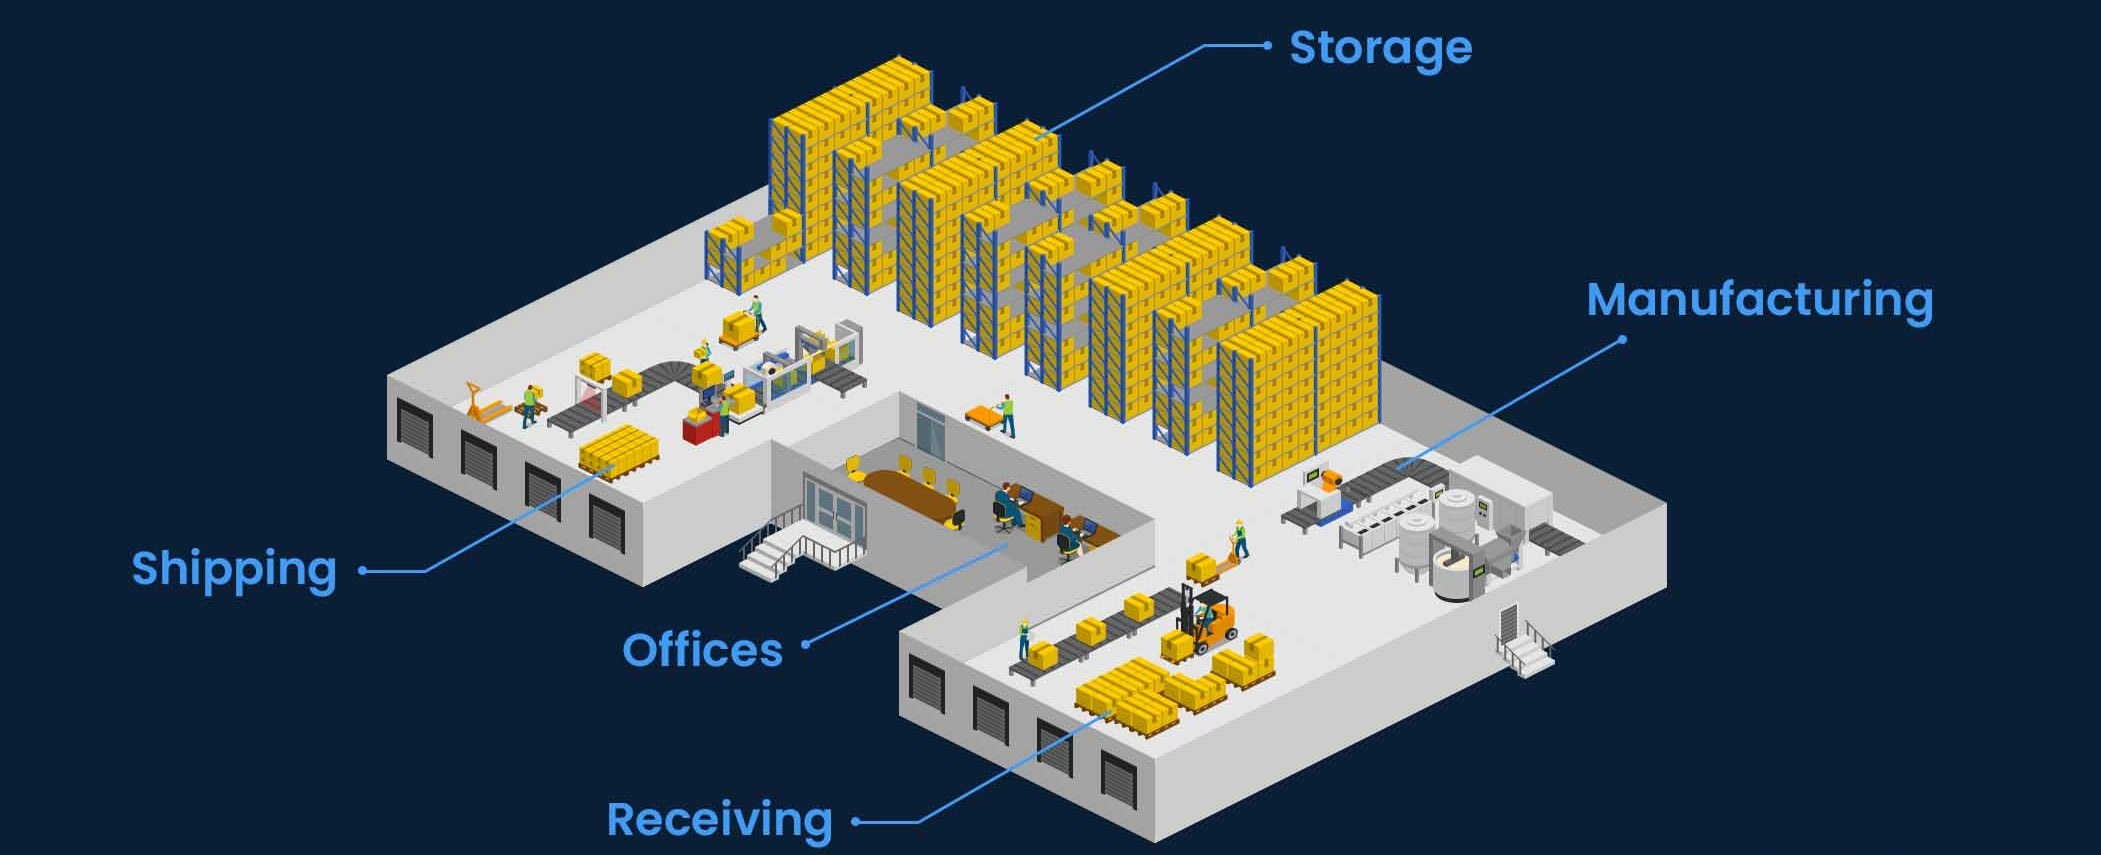
\includegraphics[width=6in]{images/Chap1/common-warehouse-areas.jpg}\\
        \caption{Common Intralogistics Environment Areas \cite{R46}}
        \label{Areas}
        \end{center}
\end{figure}

\section{AMRs in Intralogistics Environments}
Autonomous Mobile Robots (AMRs) are advanced robots designed to navigate and perform tasks independently 
in dynamic environments without the need for fixed infrastructure or human intervention. Equipped with 
sensors, cameras, and advanced software, AMRs can move around facilities like warehouses and 
factories, adjusting their paths based on real-time conditions. They are commonly used 
for material handling and transporting goods.

In the Intralogistics field, AMRs were introduced as a revolution to Automated Guided Vehicles (AGVs). 
First introduced in 1955, AGVs performed tasks like 
material handling. AGVs are managed by top-level software that handles task planning, 
providing the vehicles with intermediate waypoints to navigate from start to end points \cite{R7}.
On the other hand, AMRs are automated in a way that makes them find the solution to unexpected problems. 
Figure \Ref{AMR-VS-AGV}, shows the difference in behavior between an AMR and an AGV in the case of a 
new obstacle. While AMRs are able to surpass the obstacle through sensors recognition and obstacle 
avoidance algorithms, AGVs require human intervention to eliminate the obstacle before restarting the navigation.

AMRs fit in the cluttered ares of warehouses. Their perception of the surrounding information allows for
low commissioning efforts: they are able them to localize themselves, plan then navigate to the goal and reach their 
destinations autonomously. Their functioning does not require an expert or an engineer's intervention which 
limits the commissioning and utilization costs.

\begin{figure}[H]
    \begin{center}
       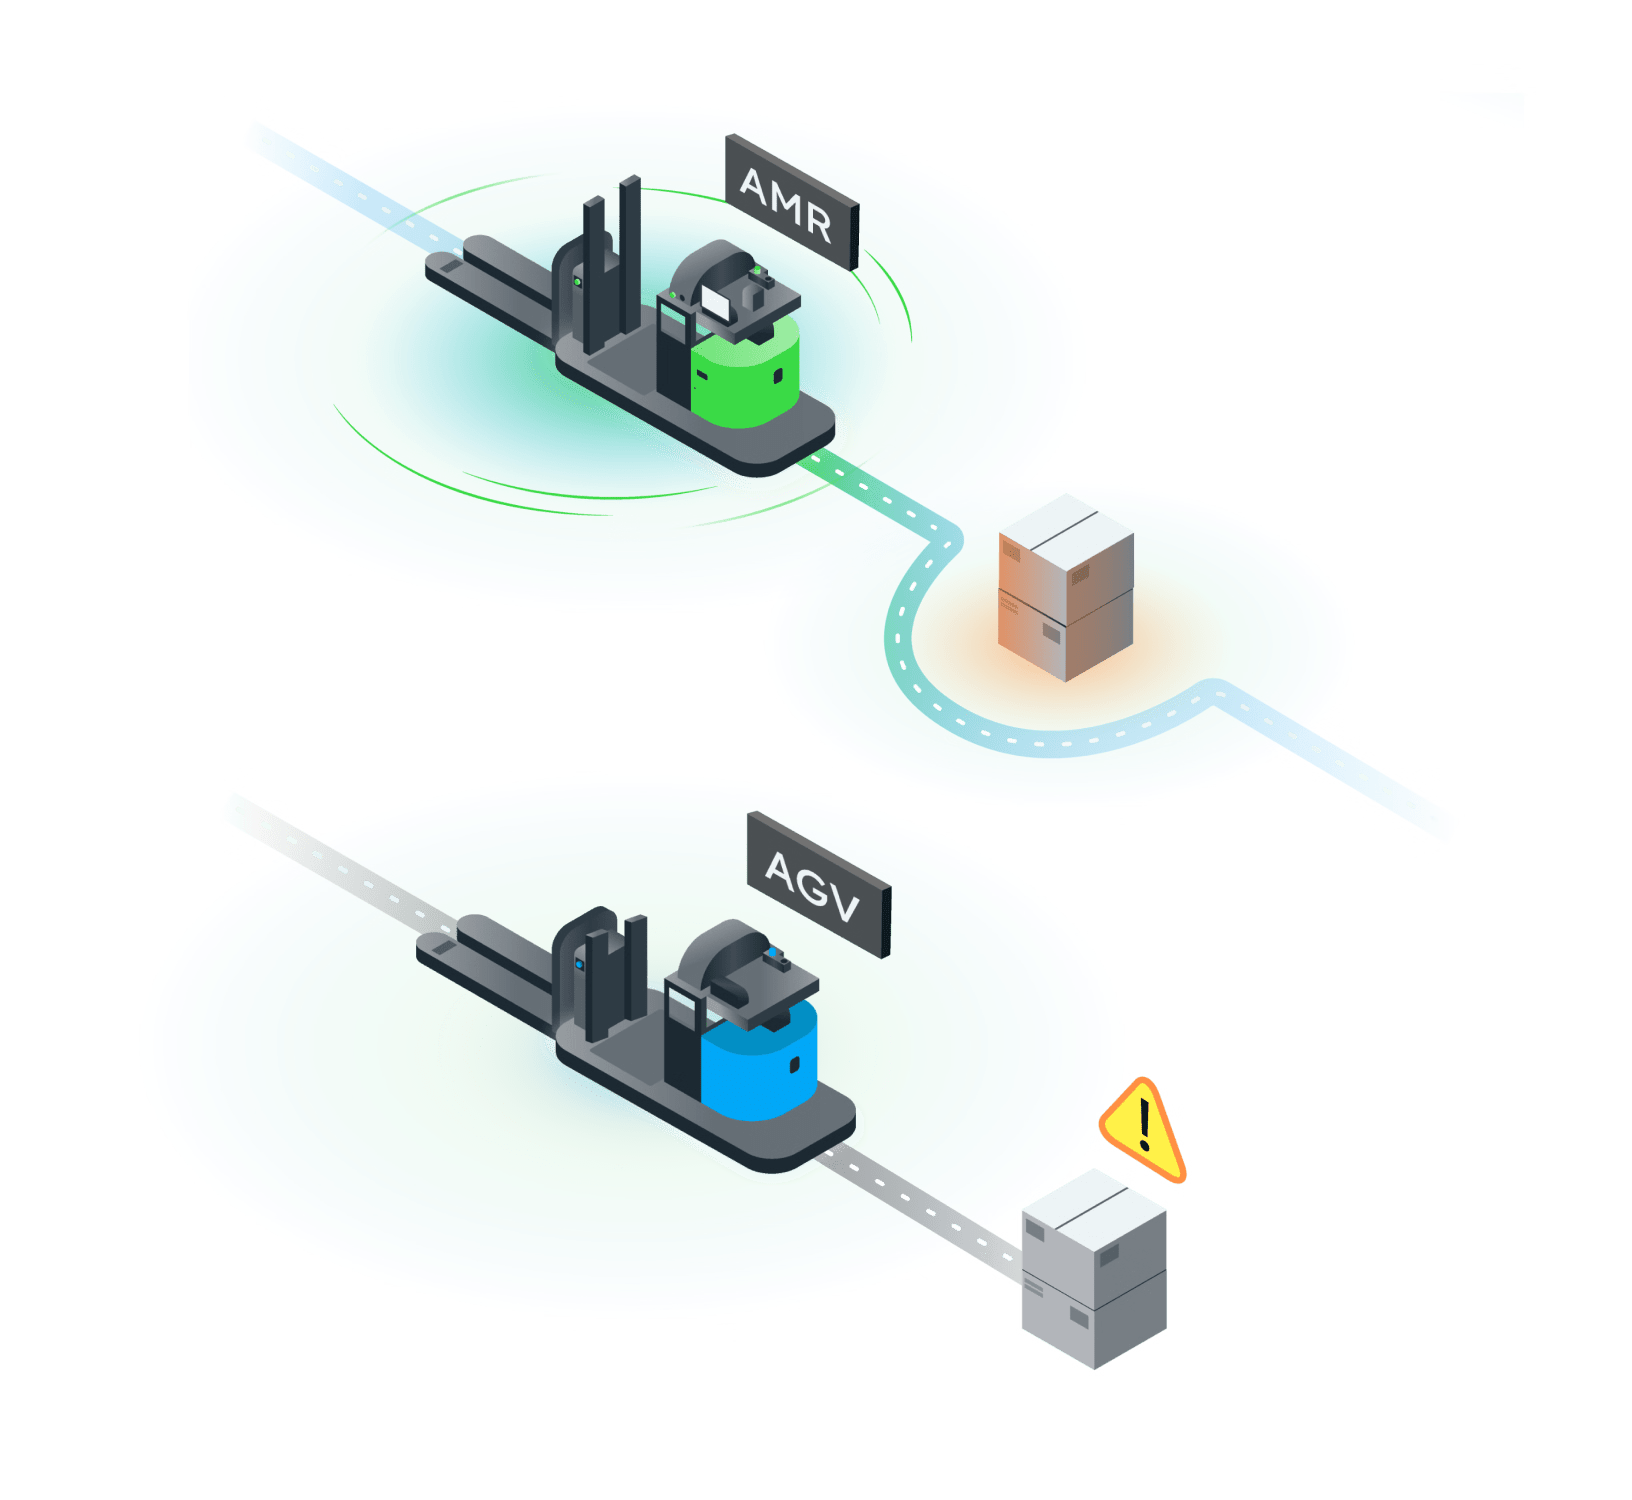
\includegraphics[width=4in]{images/Chap1/AMR-VS-AGV.png}\\
       \caption{AMR and AGV behaviors at presence of an obstacle \cite{R9}}
       \label{AMR-VS-AGV}
       \end{center}
\end{figure}

%\begin{figure}[H]
%    \begin{center}
%       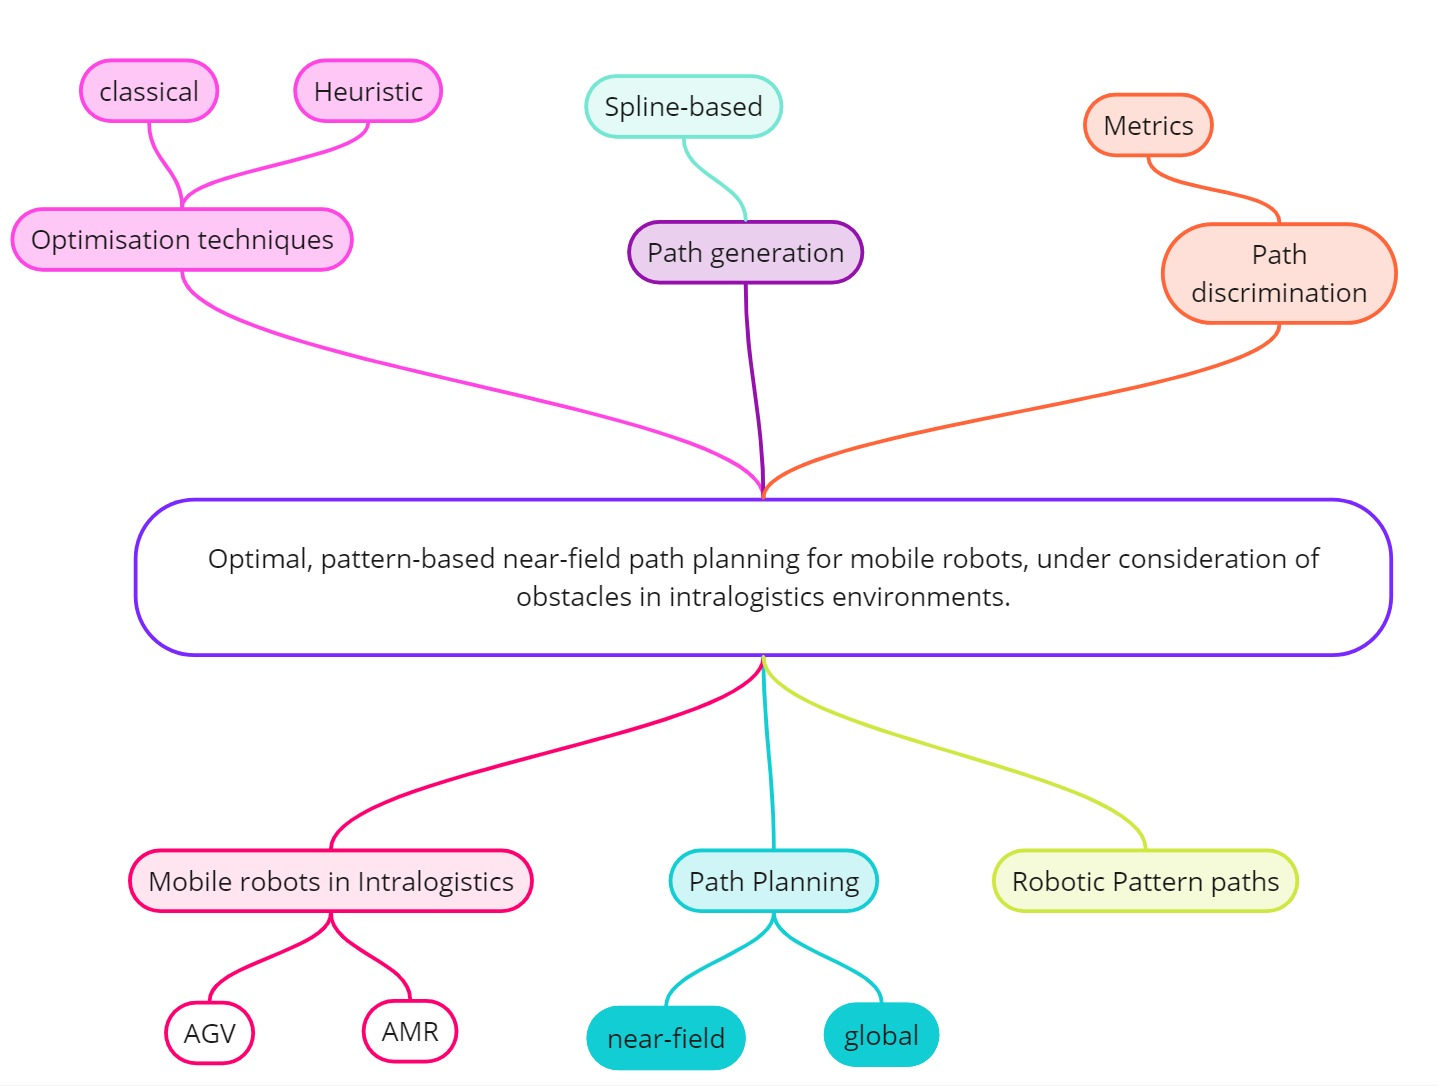
\includegraphics[width=5in]{images/Chap1/Fig1.jpg}\\
%       \caption{Mind map of the key topics}
%       \label{mindmap}
%       \end{center}
%\end{figure}

\newpage
\section{Path Planning}
This section will dive into the path planning state of the art: presenting its promising 
opportuniities and current challenges, detailing the different approaches, and discussing
their efficiency and compatibility with the problem statement.

\subsection{Path Planning for autonomous robots: Opportunities and challenges}
%opportunities
Path planning for mobile robots involves creating and generating efficient routes 
for the robot to travel from a starting position (A) to a target position (B), 
ensuring minimal time and travel distance while avoiding collisions with nearby objects \cite{R7}. Literature 
differentiates between two main types of path planning: 
global and local path planning. Global planning involves finding an optimal path from 
the start to the target position based on sensor input within a known, static environment, 
whereas local planning focuses on real-time path planning and obstacle avoidance, typically used online while 
moving to avoid dynamic obstacles \cite{R11}.

In complex environments, movement and task fulfillment must be done carefully and accurately given 
the volume of the vehicle and the value of the handled material. With appropriate input from various sensors, 
such as laser 
scanners, cameras, and LiDAR providing robots can perceive of their surrounding environment and plan the right path
accordingly. The innovation in hardware made navigation flexibility and autonomous recovery 
after failure possible\cite{R7}.
The relevance of efficient path planning, mainly in the intralogistics sector, is derived from the constant need 
of optimizing material flow, productivity rates, and cost effectiveness. Path planning reduces
travel time and distances when moving goods and thus , improving overall operational costs by allowing robots 
to take the most optimal routes when moving goods. By minimizing unnecessary detours and avoiding congested areas, 
robots can complete tasks more quickly, leading to faster material handling cycles.
In those dynamic environments (see chapter 2, section 1), operators and employees are moving around, 
goods and pallets are 
being transported or stocked, and materials must be handled safely and carefully.
Flexibility in routing and planning, enables the AMRs to always drive the optimal path
based on the space settings. This flexibility offers several benefits, such as:

\begin{itemize}
    \item Independence from Human intervention if an unexpected situation raises 
    -AMRs do not require assistance, unike AGVs \cite{R7}.
    \item Reduced energy consumption thanks to optimal: smooth and short paths that adhere to 
    the vehicles' kinematics, allocated task and travel time.
    \item Robustness and responsiveness thanks to decentralized decison making: enables fast 
    recovery and change of strategy after failure\cite{R7}.
\end{itemize}

Efficient path planning is critical for ensuring safe and reliable handling of objects in dynamic environments. 
By maintaining safe distances from both static and moving obstacles, including people, and continuously detecting 
surroundings, robots can ensure safety at all times. An optimized path improves both the length and 
smoothness of travel, minimizing travel time and boosting productivity, as tasks are repeated frequently 
throughout the day. As a result, it enhances operational efficiency, contributing to overall system 
performance.

AMRs, as the name suggests, are 
standalone systems that must compile and process such input and generate, through algorithms, 
efficient paths. Path planning serves as the crucial 
link between the robot’s sensor input and its motion control \cite{R10}.


%challenges
More that 60 years have elapsed since "Shaky" the first wheeled robot was running it first tests
in Stanford University' labs. However, most of the robotic related topic are still being researched and improved.
Dealing with all the aspects and challenges that robotics comes with can be very intricate. One of the major 
topics posing challenges to researchers is path planning. 
In a research by S. H. Tang et al. \cite{R20}, the authors reviewed recent path planning approaches and challenges
in dynamic unkown environments. 
% safety
Saftey in path planning was the main concern for 29 \% of the reviewed studies. Navigating efficient 
paths while avoiding collisions is challenging to accomplish. Collision avoidance is tightly related to perception 
input through sensors, analysis and use of the data. While it may seem simple for the robots to correctfully analyze 
and recognize the objects around them, in reality, detailed understanding is not possible \cite{R21}. Issues are 
related to the accuracy of the sensors and the robustness of the algorithms. 
It is expected from the robot to 
preceive of the obstacles just like humans do, recognizing 3d shapes, dimensions, depth, direction and velocity, 
but from the 
robot's perspective, it is only able to recognize the outer surface that reflects the sensor's luminous signals. As shown in
figure \Ref{scamSim}, the simulated robot (in gray) is surrounded by 3 obstacles (blue polygons).
While the obstacles are polygon-shaped, the perception of the robot is limited to the surfaces that 
it can scan and does not see the hidden depth beyond these surfaces.

\begin{figure}[H]
    \begin{center}
        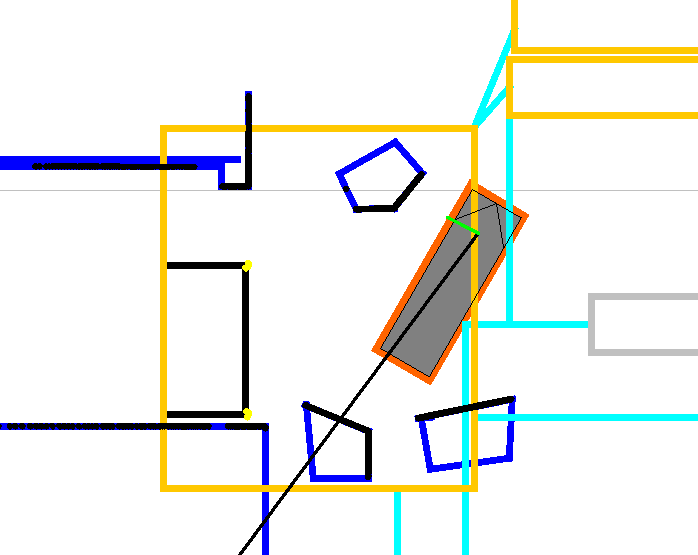
\includegraphics[width=4in]{images/Chap1/scan.png}\\
        \caption{
        Simulation of the robot's perception of surrounding obstacles.
        \newline \textbf{Yellow rectangle:} Station limits
        \newline \textbf{Black rectangle:} Shelf limits: where to pick or to place pallets
        \newline \textbf{In gray:} Robot in simulation
        \newline \textbf{Blue polygones:} Simulated obstacles
        \newline \textbf{Black lines:} Perceived obstacle points}
        \label{scamSim}
        \end{center}
\end{figure}

As a result, algorithms are to compensate the shadowed depth of obstacles by enforcing safety measures like 
keeping the vehicle at a safe distance from the obstacles and deccelerating at the proximity 
of static and dynamic objects to avoid collisions.
In addition, this input contains noises caused by the sensors reflections of other objects
or inaccuracies. 
This makes it challenging to interpret the input and create deliberative systems as the built algorithms have to 
deal with the given data
in all cases and detect the inaccuracies and noises.
Beyond that, it is complex to generate feasible solutions in all types of environments,
some planners and algorithms risk stagnating in a local minima and not converging to the optimal routes
due to the limited knowledge of the environment and the sensory limitations previously mentioned. 
Figure \Ref{local_minima} shows a simplified example of a potential wrong decision. A vehicle encounters two possible 
driving paths, similar to what might happen in a racking system. Based solely on sensor data 
(grey shaded area), the correct path cannot be determined. Only with global path planning (green path) 
can a long-term route be selected (black arrow), avoiding the risk of ending up in a dead end (red arrow). 
Assuming the global trajectory leads to the mission goal, any local deviations from this path should be 
kept minimal while avoiding obstacles.

\begin{figure}[H]
    \begin{center}
        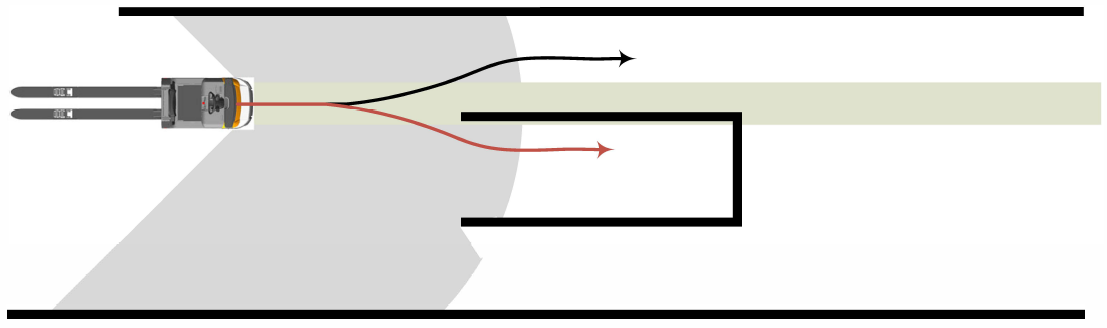
\includegraphics[width=4in]{images/Chap1/local_minima.png}\\
        \caption{Model of a local minima problem 
        due to limited sensor output \cite{R28}}
        \label{local_minima}
        \end{center}
\end{figure}

%Computational intensivity

Besides safety, computational cost is an interesting topic that researches 
are looking at. In a real time context, it is important to synchronize different tasks, 
analyze massive amounts of data generated by sensors and camera like point clouds and 2d/3d images, 
and compute the required decisions in a reliable and accurate way. As the complexity of the environment 
increases, so does the computational burden, often leading to longer processing times or the need for 
more powerful hardware \cite{R23}.

%smooth paths length and control:
While managing computational costs is crucial, it is equally important to ensure that the paths 
generated are not only computationally efficient but also smooth and short, as these factors 
significantly influence the robot's overall performance.
Given the kinematics of a robot, the destination's location and the clutter in the environment, 
path planners usually render rough paths. Cusps, which are sudden and sharp direction changes, and high
curvatures of the path are unusual path properties that are hard to drive, energy and time inefficient, 
and require continuous decelerations and accelerations. Long paths are also not favored. While they can be 
necessary to avoid obstacles or to create a smooth path, longer distances result in time consumption and 
extensive energy usage. 
Some path planner include post-smoothing methods that modify the paths after its creation and intervene by
shortening and smoothing paths areas while obstacles. In \cite{R23}, Heiden et al. present approaches 
to implement post-smoothing methods like B-Splines, Shortcuts, Simplify Max, and vertex optimization. 
They conclude that different methods deal with certain 
improvements areas differently. For example, While Splines are outperformed in the curvature and cusps 
areas, they are efficient when it comes to path-smoothning computation time.  

In conclusion, tackling robot path planning requires looking at several improvement
areas: computational intensivity, smoothing, and safety at the same time. Most path planning approaches 
are effective in the aspects that they focus on, but lack optimization in others. This further emphasizes that these 
challenges remain under research and are not yet fully addressed in the literature. While these challenges 
highlight areas needing further exploration, path planning approaches propose techniques 
to address them. Understanding these approaches can provide insights into potential solutions and 
advancements in overcoming the existing limitations.


\subsection{Near-Field Path Planning}
Path planning can be differentiated into Global Path Planning (GPP) and Local
Path Planning (LPP) or Near-Field Path Planning (NFPP). The GPP generates a global trajectory based on static and 
known environment model, such as the current pose, target location and the static components 
of the environment like shelves and walls \cite{R28}. 
The LPP generates relative trajectories and allows deviation from the previously generated global 
trajectory if disturbances in the travel path are detected. However, LPP tend to converge into local 
minima as explained in the previous section .

Due to the sheer number of publications around LPP, the work of  Kr\"uger-Basjmeleh \cite{R28} clusters 
processes into 4 groups. Figure \Ref{cluster} illustrates 4 clusters. 
The classification of the methods is done by dividing them into direction, speed, and path generating methods and 
other methods based on AI for NFPP. All methods rely equally on immediate sensory input from the 
environment as the basis for future tracking strategies.

\begin{figure}[H]
    \begin{center}
        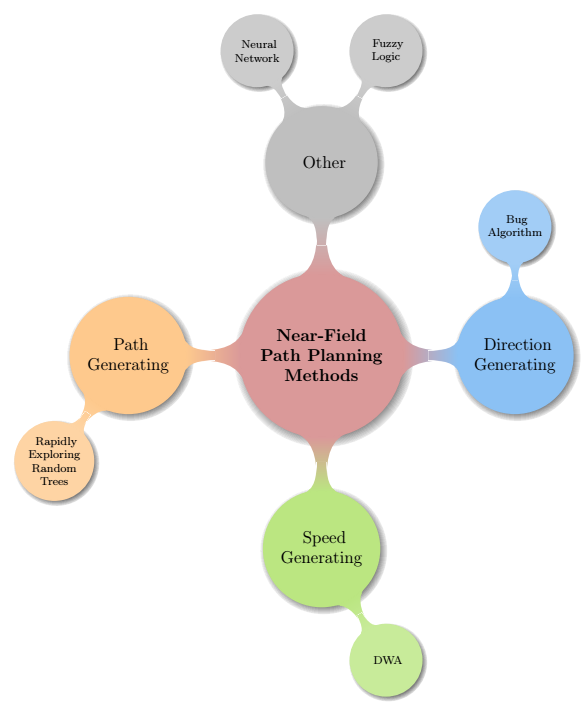
\includegraphics[width=4in]{images/Chap1/clusters.png}\\
        \caption{Clustering Of Near-Field Path Planning Approaches \cite{R28}}
        \label{cluster}
        \end{center}
\end{figure}

The process groups are then differentiated to identify their advantages, limitations and suitability 
to the problem statement. For each cluster one or two methods are studied and explained, through which 
the discrimination is made. 

\textbf{Direction-generating methods} compute feasible travel directions (directional state space) 
based on sensory input, which the AMR should follow in the next time step \cite{R28}.
A very simple algorithm for obstacle avoidance is the Bug algorithm.
In their research paper \cite{R25},
Buniyamin, N. et al. propose the point to point Bug algorithm to navigate in unkown environments. 
Bug algorithms are based on range sensors input. As illustrated by \ref{Bug_Algo}, the robot at the 
starting point (Start green dot), 
plans to move directly to the 
Goal (Goal Red dot). Then it rotates scanning for obstacle points. 
If it encounters a sudden obstacle point \((A)\), it navigates in its direction.
The robot rotates in the target's direction (\(B\) then \(C\)) until it is able to resume its direct path to 
the target based on the 
constant search for the shortest distance from the current standpoint or find the next obstacle. 

While this approach is simple from the computational point of view and the hardware used, it may not be 
optimal considering other metrics. First it can be significantly affected by sensory noises.
Besides, its path length optimality depends on the nature of the environments and the number of obstacles 
and its effciency decreases if the complexity (obstacle density) of the test area increases: in figure 
\Ref{Bug_Algo}, the path rich in vertices : start-A, A-B, B-C, and C-goal, which makes it 
long and lacks optimization.

\begin{figure}[H]
    \begin{center}
        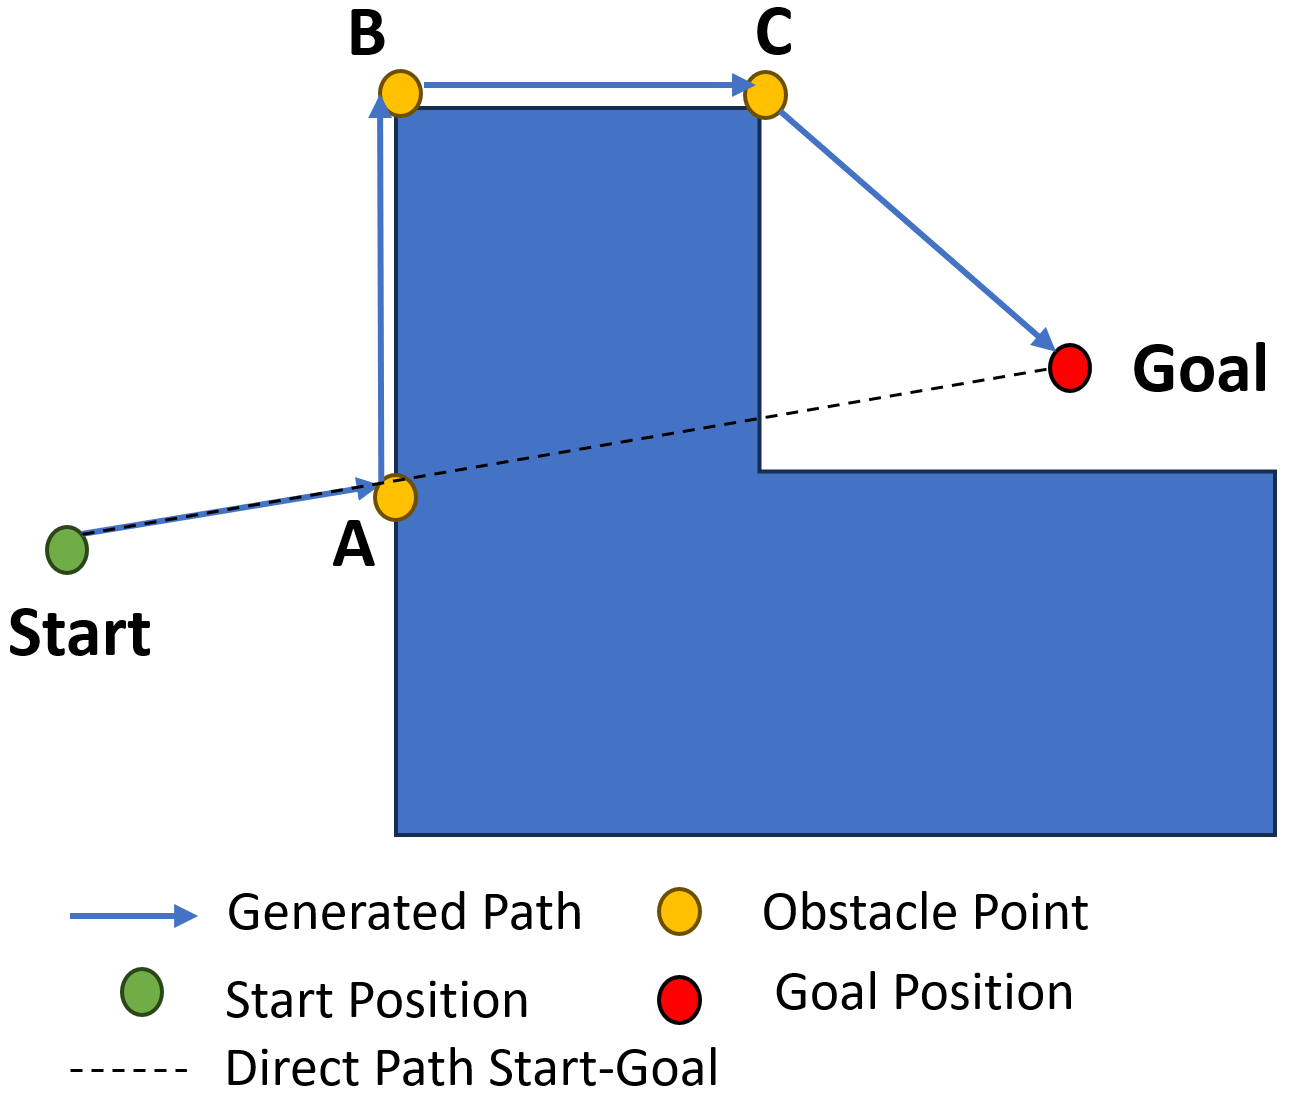
\includegraphics[width=3in]{images/Chap1/Bug_Algo.png}\\
        \caption{Bug Algorithm Path Solution to navigate from Start to Goal while avoiding
        the obstacle}
        \label{Bug_Algo}
        \end{center}
\end{figure}

\textbf{Velocity-generating path planning methods} are algorithms used in AMRs, to calculate both 
the speed and direction of movement. They predict the rotational and translational velocites 
creating the state space of velocities and taking into account the sensory inputs \cite{R28}. 
The Dynamic Window Approach (DWA) is a Velocity-generating path planning method.

In \cite{R19}, Liu et al. used Djikstra ALgorithm (A path-generating Algorithm) 
for Global path planning and 
the DWA as the local path planner for sudden unkown obstacles that could 
appear for smart cars while following the global path.
It works by evaluating different possible movements the robot could make within a short time frame 
and choosing the one that avoids obstacles while also moving towards the goal. The "window" refers 
to a limited set of possible velocities of the velocity space the robot can use based on its current 
speed and capabilities. Figure \Ref{flowchart of the DWA} details the flowchart of the DWA. 
The DWA algorithm starts by analyzing the car's position and base data. It then samples the speed and 
generates a range of possible trajectories. Each trajectory is evaluated to check if it will collide with 
obstacles. If a trajectory is collision-free, it's considered for optimal trajectory selection. This process 
continues until all possible trajectories have been evaluated or an optimal one is found.
The combined algorithms were tested on 3 spaces with 3 stages of environment complexity ranging from 
simple to complex. However, the tests were effected with dynamic obstacles only inside the simulation and
soit is subject for the reality gap problem.
While these methods excel at avoiding obstacles at high speeds, they struggle with local minima. This is 
because they don't consider the overall structure of the free space when evaluating movements.
Additionally, these velocity-generating methods have limitations in mapping the future movements of 
non-holonomic platforms. For example, a method might suggest a movement that is impossible for the 
vehicle to perform due to its non-holonomic nature \cite{R28}.

\begin{figure}[H] 
\centering  
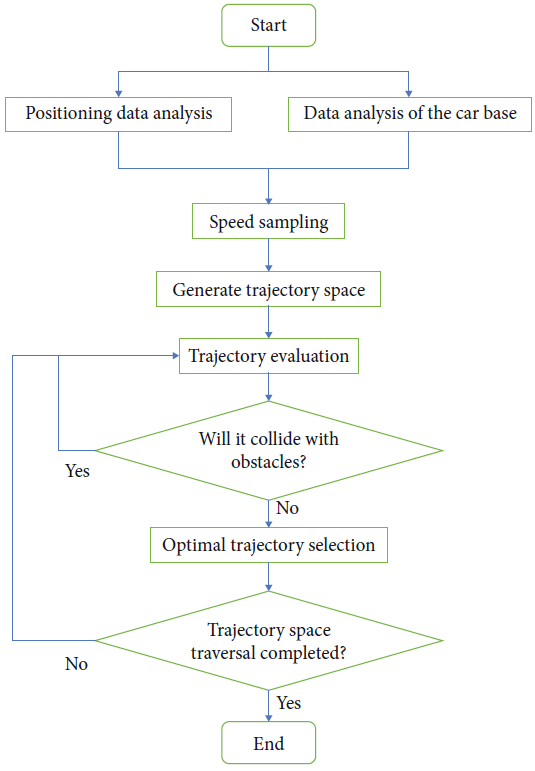
\includegraphics[width=3.5in]{images/Chap1/DWA_flowchart.png}  
\captionof{figure}{Flowchart of the DWA \cite{R19}}  
\label{flowchart of the DWA}  
\end{figure}

\textbf{Path-generating path planning methods} plan entire trajectories in advance, considering both the 
vehicle's position and its intended path over time. These planned trajectories are then combined with 
the previously calculated overall path. Currently, various path planning methods are used in both industry 
and research \cite{R28}.
For example, A* Algorithm is a Path-generating Grid-based method where
the environment is partitioned into a grid of discrete cells, where each cell represents a 
portion of the space. 
The algorithm then traverses these cells to identify suitable paths based on factors such as occupancy 
or cost. For example, in the A* algorithm, the fitness function is calculated from the start point 
to the reached cell, while in the Dijkstra algorithm, it's from the reached cell to the destination. 
While this approach offers a straightforward understanding and implementation, its computational cost 
can be significant due to the large number of cells to evaluate and the repetitive nature of the 
calculations. Additionally, grid-based methods are often constrained by the fixed directionality 
of the grid. The paths generated are restricted to the directions defined by the grid. 
For instance, if the grid is aligned along the x and y axes, the robot can only move horizontally 
or vertically. This can be inefficient or even impossible in environments where diagonal 
or more complex movements are required.
On the Other hand, 

Lavalle created a method called Rapidly-exploring Random Trees (RRT), a randomized data structure used 
for various path planning tasks. It starts with a single node (usually the starting point)
and iteratively grows a tree by adding new nodes. At each iteration, a random point is sampled from 
the search space. The nearest node in the tree is found, and a new node is added along the path to 
this random point. This process is repeated until a path is found or a maximum number of iterations 
is reached. RRT is particularly effective for exploring complex environments with obstacles. 
Figure \Ref{sampling-based}, illustrates the test of RRT in an obstacle-rich environment (shown in blue)
using 1, 4, then 32-core processors. The planned paths (branches) are shown in grey. 
The path calculated as optimal is shown in red and connects the start pose with the goal pose.
These algorithms present advantages like handling big environments and complex obstacle
situations, however, they can also be computationally intensive and demanding in complicated situations.
Figure \Ref{sampling-based} shows the difference in the resulting optimal path in a cluttered environment where with
1 core the algorithm successfully finds a feasible path, and, as the cores double, the computed path
improves its quality as the search tree expands. 
RRTs require collision checks for each new node, which can be computationally expensive and memory-intensive, 
especially in environments with numerous obstacles, heavy traffic, or complex paths.


As for artificial intelligence-based methods, also known as heuristic and metheuristic approaches, 
leverage the use of neural networks, machine learning and deep learning, and evolutionary algorithms. 
These methods learn from experience, adapt to changes, and optimize paths in complex environments. 
They are good at handling dynamic and unpredictable scenarios, making them suitable for tasks like 
autonomous driving, robot navigation, and logistics. 


\begin{figure}[H]
    \begin{center}
       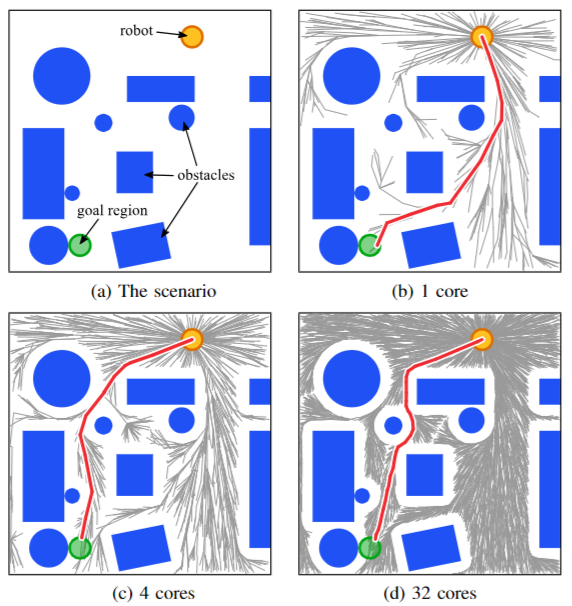
\includegraphics[width=3.5in]{images/Chap1/sampling-based.png}\\
       \caption{RRT ran on a non-holonomic robot using 1, 4, then 32-core 
       processors \cite{R16}}
       \label{sampling-based}
       \end{center}
\end{figure}

To start with, Neural networks (NN) are inspired from the biological harmonious connection of the brain neurons
that gives it the ability to process big amounts of data and generate ideas and decisions and solve problems. 
The NN is built in a way that enables it to get its input in a form of data and process it by learning, improving 
and adjusting the output to the desired results. NN are able to perform Parallel processing: the information is 
transmitted in two
directions to the neuron in the case of Recurrent Neural Networks (RNN) that allows for learning fron current and 
past inputs to the NN. This approach improves the computation time and overall performance. 
The NN is then able to process complex solutions and create paths for difficult environments. 
It is well suited for unpredictable situations as it is built to adapt to the available input and the desired output.
However, it presents a practicality challenge. Althugh the performance an results can be impressive, yet, in a 
real-time context, 
it is hard to rely on solutions that require extensive computational efforts and need long durations to 
process solutions. In addition, the number of neurons and layers have to be scalable and depends closely on the 
level of complexity that the vehicle is to deal with \cite{R12}. 

Fuzzy Logic (FL), on the other hand, is a way of thinking that mimics how humans make decisions, especially when things are unclear 
or uncertain. Instead of working with exact numbers, it uses "fuzzy" terms like "good", "average" or "bad" to make 
decisions. Input numbers are clustered following the fuzzy sets or intervals and assigned a value using membership 
functions. Later the values are interfered and defuzzified to genearte the ouput as a command value. 
In robotics and path planning, FL helps robots navigate by allowing them to handle uncertain situations, 
like avoiding obstacles or finding the best route, even when the environment is not fully known. Instead of needing 
exact data, the robot can employ fuzzy terms like "close" or "far" to understand its surroundings. For example, if an 
obstacle is "somewhat close," the robot can smoothly adjust its path to avoid it. FL also helps the robot choose the best 
route by weighing various factors like distance and safety, even when the information is not perfect. This makes the 
robot better at handling unpredictable environments and making flexible and optimal decisions.
However, one 
disadvantage is that it can be tricky to create the right rules for the robot to follow, and the system can become 
complicated as more rules are added. It may present a scalability problem because in unpredictable and dynamic environments
it is not simple to decide about fixed fuzzy sets that would be practical in all of the cases \cite{R12}.

While Neural Networks and Fuzzy Logic offer powerful approaches for handling uncertainty and complex decision-making, 
another key area in artificial intelligence for path planning is the use of meta-heuristic algorithms.
Meta-Heuristoc algorithms are inspired from biological and natural processes for evolution and survival. 
Unlike NN and FL, that rely on data as input to generate decisions, meta-heuristic algorithms explore the solution
space by evolving random solutions for the problem and optimizing them by rounds until a stopping criterion or set
of criteria is satisfied (see more in section ...: Optimization Algorithms).
Approaches like Genetic Algorithms (GA) have been used for path planning by Ahmed Elshamli et al. \cite{R17}. The The robusteness of their 
solution is its adaption to dynamic environments. They evolve their GA using variable size chromosomes, where each node 
represents a waypoint of the path, then they measure the quality of each path using an evaluation function. A modified Genetic Approach is then 
applied to each population: Crossover, mutation, \textbf{Repair} infeasible paths, \textbf{Shorten}, then \textbf{Smoothen} 
feasible paths while dynamically checking for new obstacles.
The approach is tested in static and dynamic environments and has achieved proven efficiency when it comes 
to local optima challenges and survivig the best elements of the population. While the use of the GA itself is robust
and successful, it can be challenging to recreate the algorithm and to add the improvements. In addition, the tests
the ran are limited to a simple simulation with unrealistic situations and obstacle setting as displayed in 
figure \Ref{R17 test scenarios}. 

\begin{figure}[h!]
    \centering
    \begin{minipage}{0.30\textwidth}
        \centering
        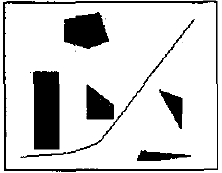
\includegraphics[width=\linewidth]{images/Chap1/R17_simple.png} % Replace with your figure
        \caption{Simple obstacle environment       }
        \label{Simple obstacle environment}
    \end{minipage}
    \begin{minipage}{0.30\textwidth}
        \centering
        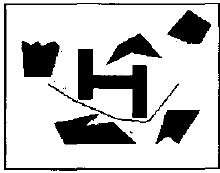
\includegraphics[width=\linewidth]{images/Chap1/R17_intermediate.png} % Replace with your figure
        \caption{Intermediate obstacle environment}
        \label{Intermediate obstacle environment}
    \end{minipage}
    \begin{minipage}{0.30\textwidth}
        \centering
        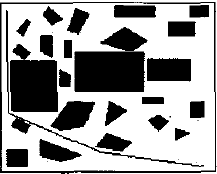
\includegraphics[width=\linewidth]{images/Chap1/R17_complex.png} % Replace with your figure
        \caption{Complex obstacle environment}
        \label{Complex obstacle environment}
    \end{minipage}
    \caption{GA Test scenarios \cite{R17}}
    \label{R17 test scenarios}
\end{figure}

\subsubsection {Local Path Planning}
Local path planning has as the role to make real-time decisions about how to move 
safely and efficiently in their surroundings. Unlike global path planning, which focuses on 
finding the best overall route from a starting point to a destination based on a static map, local path 
planning deals with navigating the environment directly around the robot while considering real-time
data input from sensors without prior knowledge about the surroundings\cite{R18}. This involves quickly 
responding to obstacles that appear or changes in the terrain, ensuring the robot can 
continue moving without collisions. Unlike Global Path planning, it functions without prior localization
and mapping of the surrounding environment. Local path planning is crucial for the safe and effective 
operation of robots, especially in 
dynamic and unkown environments. For example, in busy spaces with moving people 
or vehicles, a robot needs to be able to make quick adjustments to avoid accidents. This type of 
planning allows the robot to react immediately to new information, making it essential for applications 
where unpredictability and quick responses are vital, such as in autonomous vehicles or service robots in 
warehouses and factories.

Common Techniques involve Reactive methods which are approaches in local path planning that focus on real-time
obstacle avoidance and online adjustements on the path that are processed while the robot is navigating.
Techniques like the Potential Fields, 
Dynamic Window Approach (DWA), and Bug Algorithms are commonly used. In their research paper \cite{R25},
Buniyamin, N. et al. propose the point to point Bug algorithm to navigate in unkown environments. 
Bug algorithms are based on range sensors input. The robot at the starting point, plans to move directly to the 
target. Then it rotates scanning for obstacle points. If it encounters a sudden point, it navigates in its direction.
The robot rotates in the target's direction until it is able to resume its direct path to the target based on the 
constant search for the shortest distance from the current standpoint or find the next obstacle. 
While this approach is simple from the computational point of view and the hardware used, it may not be 
optimal considering other metrics.
Its path length optimality depends on the nature of the environments and its effciency decreases if the complexity
of the test area increases. 
Local path planning approaches are effective in navigating through cluttered environments, but when it comes to 
long-range planning, a hybrid approach that integrates both local and global path planning strategies can provide 
more robust and efficient results.

\subsubsection {Hybrid Path Planning}

In recent years, path planning approaches that combine both global and local techniques have gained popularity. 
By integrating global and local path planning approaches, robots and autonomous vehicles can take advantage of 
the strengths of both methods. This hybrid approach is a promising area of research, with the potential to benefit 
a wide range of applications. Hybrid path planning approaches are becoming increasingly popular due to their ability 
to handle complex environments and dynamic obstacles.

\noindent
\begin{minipage}{0.5\textwidth}  
    In \cite{R19}, Liu et al. used Djikstra ALgorithm for Global path planning and 
    the DWA as the local path planner for sudden unkown obstacles that could 
    appear for smart cars while following the global path.
    It works by evaluating different possible movements the robot could make within a short time frame 
    and choosing the one that avoids obstacles while also moving towards the goal. The "window" refers 
    to a limited set of possible velocities of the velocity space the robot can use based on its current 
    speed and capabilities. Figure \Ref{flowchart of the DWA} details the flowchart of the DWA. 
    The combined algorithms were tested on 3 spaces with 3 stages of environment complexity ranging from 
    simple to complex. The tests showed that the hybrid path planning approach was efficient for navigating the 
    robot and avoiding collisions. However, the tests were effected with dynamic obstacles only inside the simulation.
\end{minipage} 
\begin{minipage}{0.5\textwidth}  
    \centering  
    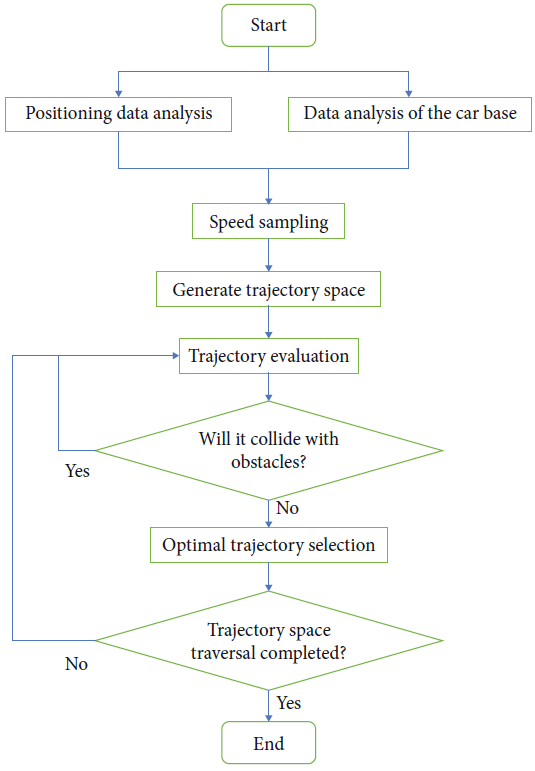
\includegraphics[width=\linewidth]{images/Chap1/DWA_flowchart.png}  
    \captionof{figure}{Flowchart of the DWA \cite{R19}}  
    \label{flowchart of the DWA}  
\end{minipage}  


Sensor-based approaches, on the other hand, rely on data collected by the robot's sensors, such as LIDAR, 
sonar, or cameras, to make decisions about where to go next. These sensors help the robot create a map of 
its surroundings, which can then be used to identify obstacles and safe paths. Occupancy grids and Point 
cloud processing are techniques used to interpret the sensor data and guide the 
robot's movements. This approach allows the robot to have a detailed understanding of its immediate 
environment, making it more capable of avoiding obstacles and navigating complex spaces.

\subsection{Discussion}

While traditional path planning methods have proven effective across various applications and usecases, 
they often face challenges when applied to highly structured, repetitive environments like those found 
in industrial automation. To overcome these limitations, the research in the previous years became rather 
oriented to investigating and using heuristic approaches. In \cite{R26}, Masehian et al. conducted a 
chronological review about the followe approaches in Motion Planning (MP). The results testify that in 30 years,
The application of Heuristic approaches in MP went from 0\% to 54\% from 1977 to 2007 as shown on Figure 
\Ref{heuristic barchart}.

\begin{figure}[H]
    \centering  
    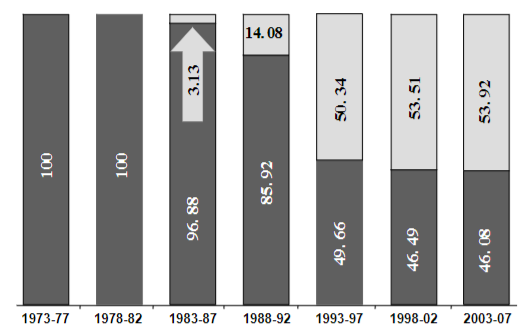
\includegraphics[width=3.5in]{images/Chap1/heuristic_barchart.png}\\ 
    \captionof{figure}{Application of classic and heuristic approaches in MP \cite{R26} 
    \newline \textbf{Dark gray:} Classic approaches
    \newline \textbf{Light gray:} Heuristic approaches }
    \label{heuristic barchart} 
\end{figure}

The classic algorithms have the drawback of traps in local minima and increased complexity in sophisticated environments.
In practice, the conditions where the robot operates are cluttered and complex than we can imagine which makes the classic 
approaches impractical. Consequently, it is necessary to tackle these issues in a different way. Although 
probabilistic methods proved high computational capabilities, scientists tend to combine 2 algorithms to 
benefit from the classic and heuristic advantages simultaneously. In \cite{R27}, Chen et al. delve into a hybrid
approach for online motion planning. Their approach is based on space exploration and heuristic search to determine 
optimal path linking a start point to an end goal. Tested on both low and high speed scenarios, the algorithm ensured
a low planning time: it outperformed RRT and had similar results in terms of planning time to Hybrid A*. 

To draw to a close, even though researches confirm that the heuristic approach prevails the classic one:
\cite{R20} and \cite{R25}, these approaches are not without their limitations. Heuristic methods, while good at 
navigating complex environments and avoiding local minima, sometimes fall short in finding the best possible 
solutions, especially in high-dimensional spaces. In contrast, classical methods, though computationally 
expensive, provide a more systematic and theoretically solid approach to path planning. To address these trade-offs, 
there is growing interest in hybrid methods that combine the strengths of both approaches. 
These hybrids use the precision and reliability of classical methods along with the flexibility and 
speed of heuristics. By doing so, they reduce the weaknesses of each approach, offering a more 
balanced and effective solution for path planning in complex environments. As a result, hybrid 
methods hold promise for future research, potentially leading to more efficient and dependable 
path planning algorithms.

\newpage
\section{Spline based Paths}
%introduction
This section will closely examine splines, their different types, their application in robotics and the 
importance of their integration and detail the challenges and limitations related to the use of Splines
for robotic motion planning, and conclude by a discussion around their relevance to this work.

\subsection{Definitions and Basic Concepts}

In mathematics and computer graphics, a \textbf{curve} is a continuous and smooth flowing line without sharp angles. 
It can be defined parametrically or implicitly and represents a path that can be traced by a moving point.
A curve can be defined using a parameter 
\(u\), where \(u\)varies over an interval, and the coordinates of the curve are given by functions of:
\begin{equation}
    C(u) = (x(u), y(u)) \quad \text{given} \quad a \leq u \leq b \label{eq:curve}
\end{equation}

The circle is an example of a curve where:

\hspace*{-1cm} % Adjust the value as needed
\begin{align}
    x(u) &= \cos(u) \\
    y(u) &= \sin(u) \quad \text{given} \quad 0 \leq u \leq \frac{\pi}{2}     \cite{R29}
\end{align}

whereas, the implicit form of the circle would be:
\begin{equation}
    (x - h)^2 + (y - k)^2 = r^2
\end{equation}

where \((h,k)\) is the center and \(r\) is the radius.


Parametric curves have a clear direction (from C(a) to C(b)), which implicit curves lack. This makes 
it simpler to create ordered sequences of points along a parametric curve. Additionally, the parametric 
form is more intuitive for designing and modeling shapes on a computer, as the coefficients in many 
parametric functions (such as Bezier and B-Splines) carry geometric significance. This results in 
user-friendly design techniques and algorithms that are numerically stable \cite{R28}. 
However, using one polynome-curves is inadequate as it is not possible to represent complex shapes, certain 
curve changes, and fitting the needed points. 
The solution is to use piecewise polynomial curves of degree \((n-1)\) for example if we need to integrate
\(n\) data points \cite{R29}.

Polynomials are a commonly used type of function in robotics because they can be easily differentiated 
and are less prone to numerical rounding errors (known as floating point errors). Although they cannot 
represent every geometric curve, polynomials can usually approximate them with sufficient accuracy. 

Using classical polynomial functions or their derivatives in Bézier form is mathematically equivalent. 
This means that any curve described using standard polynomials can be transformed into a Bézier curve, 
and vice versa. However, when it comes to geometric modeling—especially in applications like computer 
graphics or robotics—the Bézier form is often preferred. This preference is due to the fact that the 
coefficients in the standard polynomial form (also known as the power basis form) don't offer much 
information about the curve's actual shape, making it harder to intuitively control and adjust the 
curve. In contrast, the coefficients in the Bézier form -the control points- directly influence the 
shape of the curve, in a visually meaningful way, making it easier to understand and manipulate 
as shown in equation \Ref{Bezier curve} \cite{R28}. 

\begin{equation}
    C(u) = \sum_{i=0}^{n} B_{i,n}(u) \mathbf{P}_i \quad \text{with } 0 \leq u \leq 1 \label{Bezier curve}
\end{equation}

The basis function \( B_{i,n}(u) \) is called the Bernstein polynomial of degree \( n \) and follows the equation

\begin{equation}
    B_{i,n}(u) = \frac{n!}{i!(n - i)!} \cdot u^i \cdot (1 - u)^{n - i} \label{}
\end{equation}

In this context, the Bernstein polynomial is a fundamental component. 
The basis function \( B_{i,n}(u) \) is used to determine how much influence each control 
point \( \mathbf{P}_i \) has on the shape of the Bézier curve.

The geometric coefficients \( \mathbf{P}_i \) are known as control points, and they define 
the shape of the polynomial curve. In many applications, such as mapping trajectories, 
a large number of control points is needed \cite{R28}.
Furthermore, in the Bézier form, the continuity of the curve depends on the placement of 
control points. This means if you want to change the shape of part of the curve while keeping 
the rest smooth, you can't easily do so because changing one part affects the whole curve \cite{R29}.

Instead, a more effective curve representation can be expressed as:

\begin{equation}
    C(u) = \sum_{i=0}^{n} N_i(u) \mathbf{P}_i
\end{equation}

where:
\begin{itemize}
    \item \( \mathbf{P}_i \): the control points
    \item \( N_i(u) \): the piecewise polynomial functions
\end{itemize}
The continuity of the curve is determined by these basis functions, allowing for flexible modification of 
control points without affecting the curve's smoothness \cite{R29}.

The basis functions for B-splines are defined recursively. For a given degree \( p \) and a set of non-decreasing knot values 
\( \{ u_i \} \), the basis functions \( N_{i,p}(u) \) can be defined as:

\begin{equation}
    N_{i,0}(u) = 
\begin{cases} 
1 & \text{if } u_i \leq u < u_{i+1} \\
0 & \text{otherwise}
\end{cases}
\end{equation}

\begin{equation}
N_{i,p}(u) = \frac{u - u_i}{u_{i+p} - u_i} N_{i,p-1}(u) + \frac{u_{i+p+1} - u}{u_{i+p+1} - u_{i+1}} N_{i+1,p-1}(u)
\end{equation}


With:
\begin{itemize}
    \item \( u \) is the parameter along the curve.
    \item \( u_i \) are the knot values, which divide the parameter range into intervals.
    \item \( N_{i,p}(u) \) are the B-spline basis functions of degree \( p \).
\end{itemize}

In figure \Ref{NURBS} stands an example of a NURBS spline generated through setting random 
control points using th NURBS generator \cite{R32}

\begin{figure}[H]
    \begin{center}
    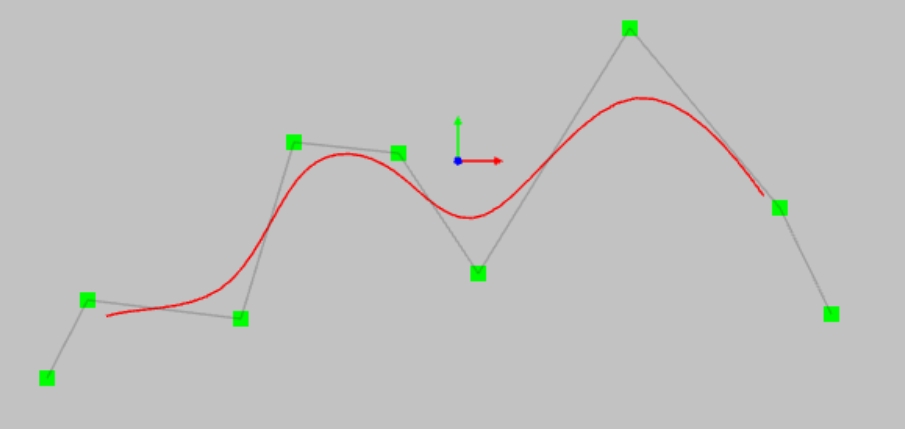
\includegraphics[width=4in]{images/Chap1/control-spline.png}\\
    \caption{NURBS spline example.\\
    \textbf{Green}: Control points\\
    \textbf{Red}: NURBS spline}
    \label{NURBS} 
    \end{center}
\end{figure}

Understanding these principles is essential as we move forward to explore the applications of splines 
in robotics. In the next section, we will examine how these spline concepts are applied to solve 
real-world problems in robotic path planning and motion control.

\subsection{Applications of Splines in Robotics}
\subsubsection{Trajectory Planning} 
%How splines facilitate smooth and continuous trajectory planning.
Robots like AMRs in the intralogistics sector usually have mission to carry heavy loads. 
This property makes it risky to operate abrupt motion changes like stopping or turning.
These vehicles' motion planning requires precise control and detailed alignment to the 
kinematic constraints that they present \cite{R30}.
Given the mathematical nature of B-Splines, they ensure continuity of the first and second derivatives.
This continuity translates to smooth transitions of the resulting velocities and accelerations of the path
that the robot will follow. By having continuous velocity and acceleration, we make sure that the robot
achieves smooth transitions and speed changes. Furthermore, tracking, precise following and correct control
interventions are guaranteed allowing for precise navigation \cite{R30}. 

 
Although simple,
the connected waypoints approach comes with drawbacks like sub-optimal travel time, unoptimized long paths, 
and mechanical wear because of abrupt direction changes unlike curved paths \cite{R30}. The morphological 
difference in both paths is distinguished in figure \Ref{paths} 

\begin{figure}[H]
    \begin{center}
        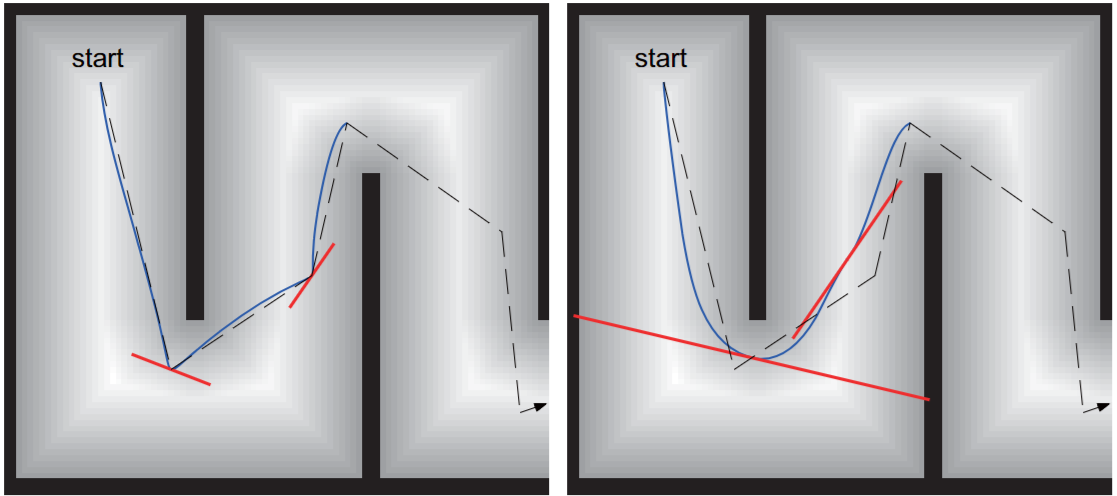
\includegraphics[width=4in]{images/Chap1/sharp-vs-curved-path.png}\\
        \caption{Morphological difference between a path connecting waypoints (left) and a curved path 
        (right) \cite{R30}}
        \label{paths}
    \end{center}
\end{figure}

Multiple approaches have been developed to introduce smooth transitions and turns into robot trajectories. 
One such method involves using Clothoid curves, which connect straight path segments with circular arcs 
to avoid abrupt changes in direction \cite{R31}. Originally introduced for designing highways and roads to 
ensure safe and comfortable driving for humans, Clothoids offer a gradual change in curvature.

However, when applied to robotics, Clothoid curves present certain drawbacks. These include the potential 
for discontinuities in curvature at the transitions, which can lead to jerky motions in robotic paths. 
Additionally, Clothoid-based paths can result in sub-optimal path lengths, as they may not be the shortest 
possible routes. Moreover, while circular arcs with constant radii are used in this approach, longer 
arcs lead to larger curvatures, which can be impractical for mobile robots that require tighter turns 
and more precise control \cite{R31}.

%Techniques for smoothing rough paths generated by planners.
Migrating from a path with sharp angles to one with smooth curves can be effectively accomplished by 
using splines. The interpolation of the control points of the original path 
creates a smooth, continuous curve. By incorporating a convex hull around these control points, we 
ensure that the path does not deviate excessively from the desired points, thus avoiding potential 
collisions with obstacles \cite{R33}. The convex hull acts as a boundary that keeps the spline inside the limits of 
the control points that prametrize it (see figure \Ref{convex-hull}) and keeps the robot from straying 
too far, ensuring a safe and accurate trajectory \cite{R29}.

\begin{figure}[H]
    \begin{center}
        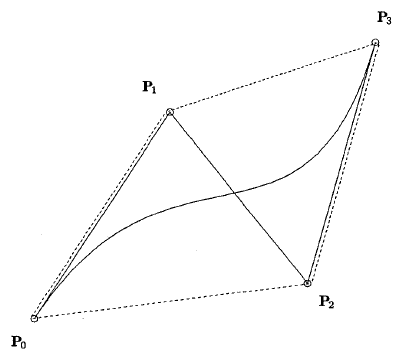
\includegraphics[width=3in]{images/Chap1/convex-hull.png}\\
        \caption{Convex hull contained Spline \cite{R29}}
        \label{convex-hull}
    \end{center}
\end{figure}

Splines are advantageous because they can accommodate various constraints such as curvature limits 
and minimum turning radii. These constraints are crucial in many applications, including robotics 
and vehicle navigation, where maintaining a smooth path is essential for stability and control. 
By adjusting the spline parameters, it is possible to design paths that meet specific requirements, 
ensuring that the resulting trajectory is not only smooth but also feasible given the physical and 
operational constraints \cite{R30}.

In scenarios involving obstacle avoidance, splines can be blended or connected to create a seamless 
path while circumventing obstacles. This blending technique allows for the integration of different 
spline segments into a continuous trajectory, ensuring that the path remains clear of obstacles. 
By carefully adjusting the blend points and ensuring smooth transitions between splines, it is 
possible to navigate complex environments safely and efficiently. This approach combines the 
advantages of smooth path planning with effective obstacle avoidance.

%Case studies of spline-based trajectory planning in autonomous vehicles.

A notable case study of splines integration in solving path planning problems, is a research conducted 
by B. Lau et al. \cite{R30} that aims to develop a time optimal solution while considering the kinodynamic 
properties of a mobile robot. They used a global planner to generate straight-line paths and minimize time 
of travel. Then, they  integrated splines to join the resulting path segments in a smooth and continuous 
way and replan in case of unprecedented collisions. The results show that our motion planning system works 
well in both real and simulated settings. It created smooth and accurate paths, with an average positional 
error of about 1 cm and a velocity error of less than 2 cm/s. The optimization process improved travel 
time by 31\% compared to initial paths. The system also handled dynamic environments, like crowded trade 
shows, and adjusted smoothly when localization errors occurred by updating the path as needed. Overall, 
it performed reliably, navigating precisely and adapting effectively to changes and errors.

\subsection{Discussion}
In general, Splines are an effective tool that centralizes advantages related to path smoothness, 
simplicity of constraining the path according to the kinodynamic properties and mechanical limitations of the 
mobile robot like limiting the curvature, and allowing for safe and smooth speed and direction changes. 
These properties accommodate simple manipulation of splines for path planning and tracking of path properties.
As an illustration, it is possible to measure the spline's features like curvature or approximate its length.
Figure \Ref{curvature}, shows an example plot of the curvatures of 3 random splines.

\begin{figure}[H]
    \begin{center}
        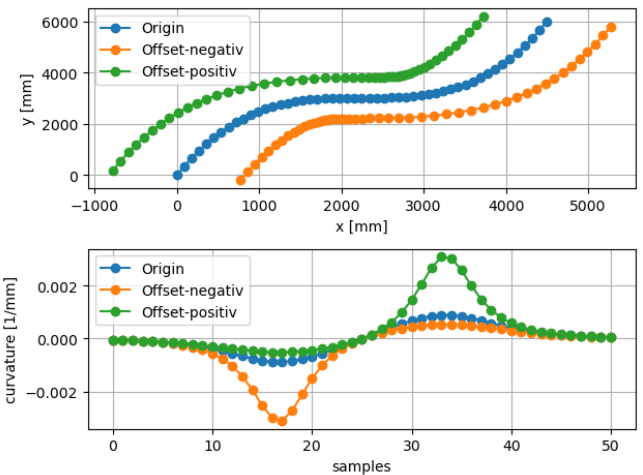
\includegraphics[width=3.5in]{images/Chap1/curvature.png}\\
        \caption{Curvature of 3 S-shaped splines}
        \label{curvature}
    \end{center}
\end{figure}
In the next section, we discuss the ways we can use such information about splines to measure paths quality.

\section{Evaluating Path Efficiency: Key Metrics}

When planning paths for robots in the Intralogistics or in any field in general, it is important to have the ability 
to quantify the quality of the resulting path. There exists different ways to judge the efficiency of the solution
and to which extent it accomodates the goal and optimizes the gaps that we are willing to improve.
This section studies the strategies that the literature followed while quantifying path quality in the robotics
field. It will look at the different indicators, why, and in which case they were used. 

\subsection{Core Metrics for Path Evaluation}
The key metrics that researchers focus on and try to improve can vary depending on the specific areas of 
optimization they are working on. For example, if the goal is to make a robot move faster, then time 
and speed might be the main metrics they study. On the other hand, if the focus is on making the robot 
navigate more safely, then the proximity to obstacles and collision avoidance would become the primary 
metrics. Therefore, the choice of metrics is closely linked to the particular goals that researchers 
aim to achieve in their optimization efforts.

According to Tang, S. H. et al. \cite{R20}, from 2011 to 2015, the second most common topic in the path 
planning research scope was path length. Path length is a key metric that helps us understand other 
important factors like travel time and energy consumption. By measuring the length of a path, we 
can get insights into how long it will take to travel and how much energy the robot might use. 
In other words, path length often reflects the overall efficiency and effectiveness of the route. 
Heiden, E et al. \cite{R23}, employed path length as of the metrics used to evaluate the length of 
the paths generated by the algorithms that they compared against each other. Their planners 
were configured to minimize path length, therefore, they measured the path lengths that were computed 
in 4 scenarios with applied to 17 path planners and 4 steering algorithms. They used path length,
along other metrics, to quantify the quality of paths after palnning and smoothing.
Besides, they compared the algorithms using the above-mentioned metrics in order to classify them
under the benchmark and to justify the choice of the best algorithm.  

In addition to path length, Path smoothness is crucial for robotics in general and especially 
in the intralogistics sector because it directly affects the efficiency and safety of robot 
operations. Smooth paths reduce the need for sudden stops or sharp turns, which helps robots 
maintain a steady speed and avoid unnecessary wear on their components. In intralogistics, 
where robots often work in busy environments with other machines and human workers, smooth 
paths also minimize the risk of accidents and product damage. Overall, ensuring path 
smoothness helps robots operate more reliably and effectively, leading to faster and 
more accurate material handling. Path smoothness reflects less cusps -sharp turns- and generally
less curvature which allows for smooth driving and smaller scale steering.
Curvature of a circle at a point \(x(t)\) is defined according to Gary D. Knott, in his book 
"Interpolating Cubic Splines" \cite{R34}, as the reciprocal of the radius at the same point as shown in
equation \Ref{kurv}.

\begin{equation}
    \kappa = \frac{1}{R}
    \label{kurv}
\end{equation}

For a cubic spline \( y = f(x) \), the curvature \( \kappa \) at a point \( x \) is given by:

\begin{equation}
\kappa = \frac{|f''(x)|}{\left(1 + \left(f'(x)\right)^2\right)^{3/2}}
\end{equation}

The unsigned curvature indicating whether the curve is concave or convexe is given by:
\begin{equation}
    \kappa = \frac{f''(x)}{\left(1 + \left(f'(x)\right)^2\right)^{3/2}}
\end{equation}

Heiden, E et al. \cite{R23}, also relied on curvature to determine path quality. They used it along 
path length and tracked it for the different scenarios and algorithms to measure their effectiveness.
Liu, S. et al. integrated path smoothness metric to quantify path quality for their benchmark to compare
motion planning algorithms\cite{R35}.
Although the above-mentioned sources used the metrics to evaluate their optimized solutions,
they did not mention the techniques  followed to measure the metrics.

Path clearance is another significant metric used to evaluate how well a robot can safely navigate 
its environment. It measures the distance between the robot's position along the path and any obstacles 
it might encounter. A larger path clearance means the robot has more space around it, reducing the risk 
of collisions and making the path safer. This metric is especially useful when optimizing paths, as it 
helps ensure that the robot can move smoothly without bumping into objects or other robots. 
Elshamli, A. et al. \cite{R17} have used path clearance as one of the indicators of path feasibility.
Clearance is measured as follows in \Ref{clear}:

\begin{equation}
    \sum_{i=1}^{n-2} \exp\left(a \cdot (g_i - \tau)\right)
    \label{clear}
\end{equation}

where \(g_i\) is the shortest distance from the \(i^{\text{th}}\) discrete position of the 
robot to the surrounding obstacles, and \(\tau\) is the desired clearance distance that 
guarantees safety. By focusing 
on path clearance, we can design routes that not only get the robot from one point to another efficiently 
but also do so in a way that minimizes risks and improves overall safety.

\subsection{Combinations of single metrics}

Some applications focus solely on minimizing path length. They use this single value as the 
metric for evaluating and distinguishing path solutions or for optimization. However, other 
applications require the combination of several metrics. This combination invites us to look 
at possible ways to blend the measured value into one significant value that reflects path quality.
Elshamli, A. et al. \cite{R17} used a weighted sum of the Distance between two nodes, or two waypoints,
Path smoothness, and clearance as given by \Ref{evaluation}. 

\begin{equation}
    \text{eval}(p) = w_d \cdot \text{dist}(p) + w_s \cdot \text{smooth}(p) + w_c \cdot \text{clear}(p)
    \label{evaluation}
\end{equation}
The outcome of this evaluation function of each path is used as the fitness function for that path.
The fitness of each path serves later the evolution of the genetic algorithm.

Zhang B et al. \cite{R36}, deployed a nonlinear optimization problem that integrates path length and 
curvature variation over a spline-based path. The problem is constrained by the curvature limits, the 
parametrized location of the spline's control points, and the distance to obstacles.

Combining metrics for path evaluation should be done with a simple approach. It is advisable to limit 
the number of combined metrics to 2 or 3. Using more metrics can make the optimization process complex 
and slow, as the optimizer has to handle more variables. Additionally, with too many metrics, it becomes 
challenging to understand how each one influences the results. By keeping the metrics to a 
manageable number, we ensure that the optimization remains efficient and the impact of each metric 
is clear and easy to interpret. 
Using a more metrics like computational time, number of cusps or direction changes, solvability percentage
or predicted speed or travel time can be efficient for evaluating path planning algorithms and benchmarking some
usecases as in \cite{R23}.

\newpage

\section{Heuristic Approaches to Path Optimization in Robotics}
%intro
This section will focus on the Application of heuristic algorithms for solving robotic path planning 
problematics. 

\subsection{}
Optimization refers to the decision making led by the machine with availability of certain circumstances and constraints
thet either help or limit the outcomes of the optimizer \cite{R37}. In the case of path planning, optimization aims
to modify some properties of the generated solutions to cope with the surrounding conditions.
In stochastic environments, it is challenging to plan feasible paths.
The increase in the complexity of the environment and the constant dynamics increase the number of variables involved 
in the mathematical representation of the problem. As a consequence, it raises the computation efforts that need to be 
deployed for the creation and optimization of the solution and decreases feasibility \cite{R7}.
The integration of an optimizer that takes charge of the solution and fits it into the constraints that bound it is necssary.
In order to get optimal results like smooth and short paths, finding a feasible path is not enough. The evaluation 
of the generated path and the optimization are helpful to ensure that the robot is driving the optimal path.
There exists a range of planners and optimizers which are clustered as classic and Heuristic approaches \cite{R12}.
Classic approaches include \textbf{Analytical} and \textbf{Enumerative} methods. 
The former rely on mathematical modeling, which can become increasingly complex as the navigation environment becomes more 
cluttered. Additionally, applying these models can be challenging in scenarios where the necessary models for different 
components are not readily available. The latter have the drawback of increased intricacy in bigger or more elaborate 
search spaces. On the other hand, Heuristic approaches can be sub-categorized into \textbf{Meta-Heuristic} and \textbf{Evolutionary algorithms}.
Some of these methods can fall in the trap of local minima and sub-optimality \cite{R12}
Alternatively, sebsequent to a review of the available planning and control approaches in intralogistics, Fragapane, G. et al. \cite{R7}, 
concluded that nature-inspired algorithms can instill intelligence into planned paths.
Elshamli, A. et al. explained in \cite{R17}, that Meta-Heuristics are adaptive to the dynamics of the surroundings
unlike classic approaches that proceed sequentially to generate solutions. The paths developed by classic approaches
can thus become infeasible in a later stage if the environment changes. Metaheuristic approaches are based 
on parallel search mechanisms that can have updated input of the conditions and thus are more adaptive and 
practical in real-world scenarios.


\subsection{Heuristic Optimization Algorithms : An Overview}
In this section, we will dive into Meta-Heuristics which are defined by Bilal et al. as 'the optimization
techniques mainly based on function evaluation and make little
or no use of the properties of objective functions and constraints.
Meta-heuristics are thus problem independent techniques not taking
advantage of any specificity of the problem’ in their review \cite{R37}.
The authors later break down Meta-Heuristics into \textbf{Neighborhood-based Algorithms} and \textbf{Population-based Algorithms}
as given by the tree graph in Figure \ref{Tree}

\begin{figure}[H]
    \begin{center}
        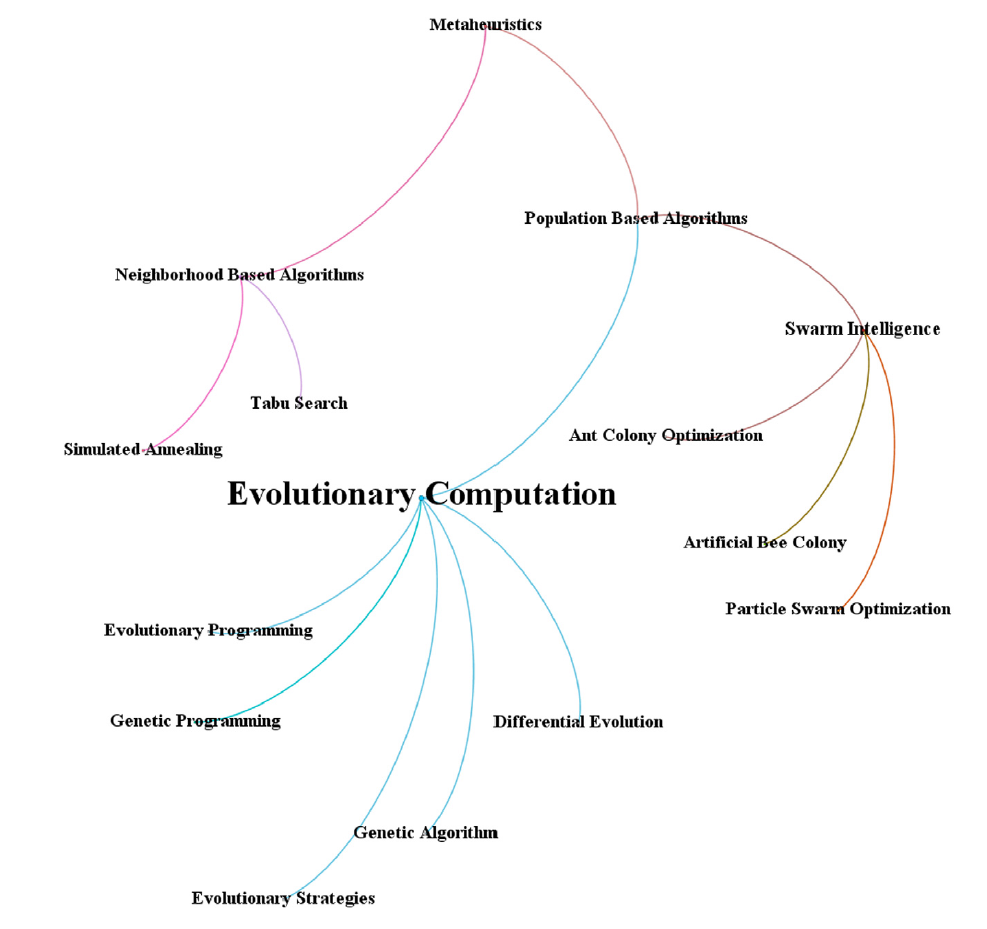
\includegraphics[width=4in]{images/Chap1/Tree_Metaheuristic.png}\\
        \caption{Tree of Meta-Heuristic Algorithms \cite{R37}}
        \label{Tree}
    \end{center}
\end{figure}

The Neighborhood-based algorithms benefit from the neighboring solutions by migrating from the current solution to 
the near surrounding solutions with the goal of improving the fitness function. The examples mentioned for this 
approach are Simulated Annealing (1979) and Tabu Search (1989). The Population-based algorithms are methods that start from a sample population and rely on their evolutions. 
They are inspired by the evolutionary processes observed in nature and are sub-categorized in this approach under 
Swarm intelligence and Evolutionary Algorithms. 
Swarm Intelligence approaches are analogous to the socio-cooperative practices of species like bees, ants, and birds. 
For instance, Ant Colony Optimization (1992)and Particle Swarm Optimization (1995) are examples of such algorithms. 
On the other hand, Evolutionary algorithms rather copy the species evolution theory, among which are Differential 
Evolution (1995) and Genetic Algorithm (1957) \cite{R37}.

\subsection{Application of Heuristic Optimization in Robotic Path Planning}
These algorithms have been used multiple times for robotic path planning, as noted in the literature. 
Each algorithm has its own unique search methods and strengths, providing different benefits and areas for optimization.
  


\begin{wrapfigure}{r}{0.3\textwidth}
    \centering
    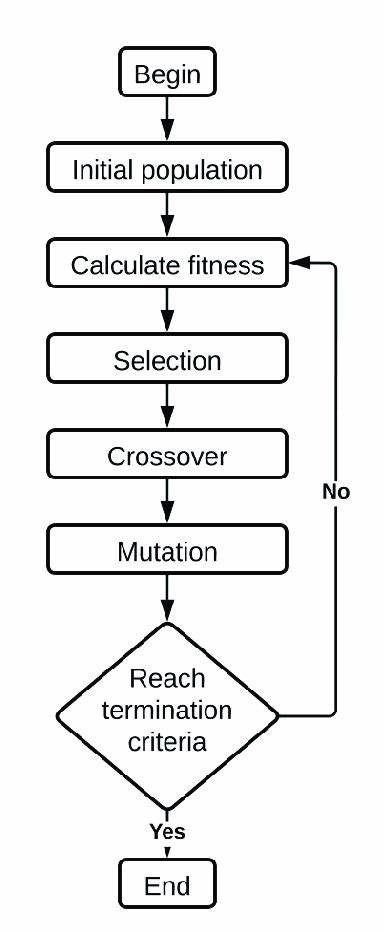
\includegraphics[width=0.25\textwidth]{images/Chap1/GA.jpg}
    \caption{Flowchart of the GA \cite{R39}}
    \label{GA}
\end{wrapfigure}

Elshamli, A. et al. \cite{R17} have employed the Genetic Algorithm (See algorithm steps in figure \Ref{GA}) to solve 
the problem of path planning in dynamic environments. They represent their paths using chromosomes where each node of the chromosome represents 
a waypoint and develop a variable chromosome length approach that accommodates obstacle avoidance and efficiency 
in reaching the goal. The fitness of each chromosome is evaluated according to an objective function that includes path length, smoothness, 
and clearance to obstacles. A modified genetic Algorithm is applied where after crossover and mutation, paths are 
shortened and smoothed if it is possible. The implemented strategies guaranteed low convergence for the different 
complexity stages. Saving the best individuals generated by the GA was effective in delivering the overall best solutions.
Tamilselvi, D. et al. also modified the GA by applying the elitism concept. They save the best solution
\(S_{best}\) then they replace the worst element of the next population with \(S_{best}\). This approach guarantees
landing on a global optimum and was able to find feasible paths for environments with limited 
dynamic obstacles and integrate a motion prediction mechanism for dynamic obstacles based on the grid map \cite{R38}.

Miao, H. et al. also worked on the path planning in dynamic environments problem. They crtic the GA to be computationally
intensive and to require long planning time \cite{R40}. Instead they suggest the Simulated Annealing algorithm (SA)
to solve the path finding problem. 
\newpage 
\begin{wrapfigure}{r}{0.45\textwidth}
    \centering
    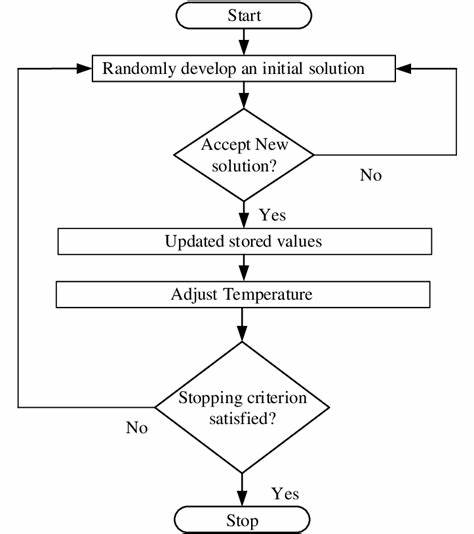
\includegraphics[width=0.4\textwidth]{images/Chap1/SA.jpg}
    \caption{Flowchart of the SA \cite{R41}}
    \label{SA}
\end{wrapfigure}

Being a probabilistic meta-heuristic algorithm it is designed to guide the local
optimum to a global optimum. The approach is based on the evaluation of the path length to discriminate 
path candidates: the shorter the path the better. It works by trying out different paths for the robot, beginning 
with a high "temperature" that lets the algorithm accept both good and bad paths. This helps it explore a wide range of 
options and avoid getting stuck in a local minima. As the process continues, the temperature slowly decreases, 
making the algorithm less likely to accept bad paths, and helping it to focus on finding the global minima as given by 
figure \Ref{SA}. algorithm was tested in four environments with different static and moving obstacles. The algorithm 
successfully found the best or nearly best paths and could quickly adjust to avoid collisions in real-time. 
Compared to a genetic algorithm, the SA method was 57\% faster for complex environments and 74\% faster for simple
environments. However, the processing time increases exponentially for complex environments (13.57 seconds).

Particle Swarm Optimization Algorithm (PSO), as well, is used for solving non-linear optimization problems like scheduling, power 
management and also robotic path planning. It is inspired from the cohesive behavior of bird and fish swarms traveling 
together.It works by having a group of particles (potential solutions) move around in the search space to find the best 
solution. Each particle in the PSO algorithm remembers the coordinates of the best solution it has found so far, known 
as its personal best (pbest). Additionally, the algorithm tracks the best solution found by any particle, referred to as 
the global best (gbest). The core idea of PSO is to guide each particle towards both its pbest and the gbest positions:
from state a to c as given by figure \Ref{pso}, 
using a randomly weighted acceleration during each iteration. The algorithm iteratively updates the particles' positions 
and velocities until an optimal or near-optimal solution is found.
Alaliyat, S. et al. have investigated dynamic environment navigation using PSO. They found out that the performance 
of the algorithm depends on parameters tuning. Overall, feasible paths were successfully generated.
Planning time is rather high for simply organized environments (18.35s) and higher for the most complicated scenario
(31.17s).

\begin{figure}[H]
    \begin{center}
        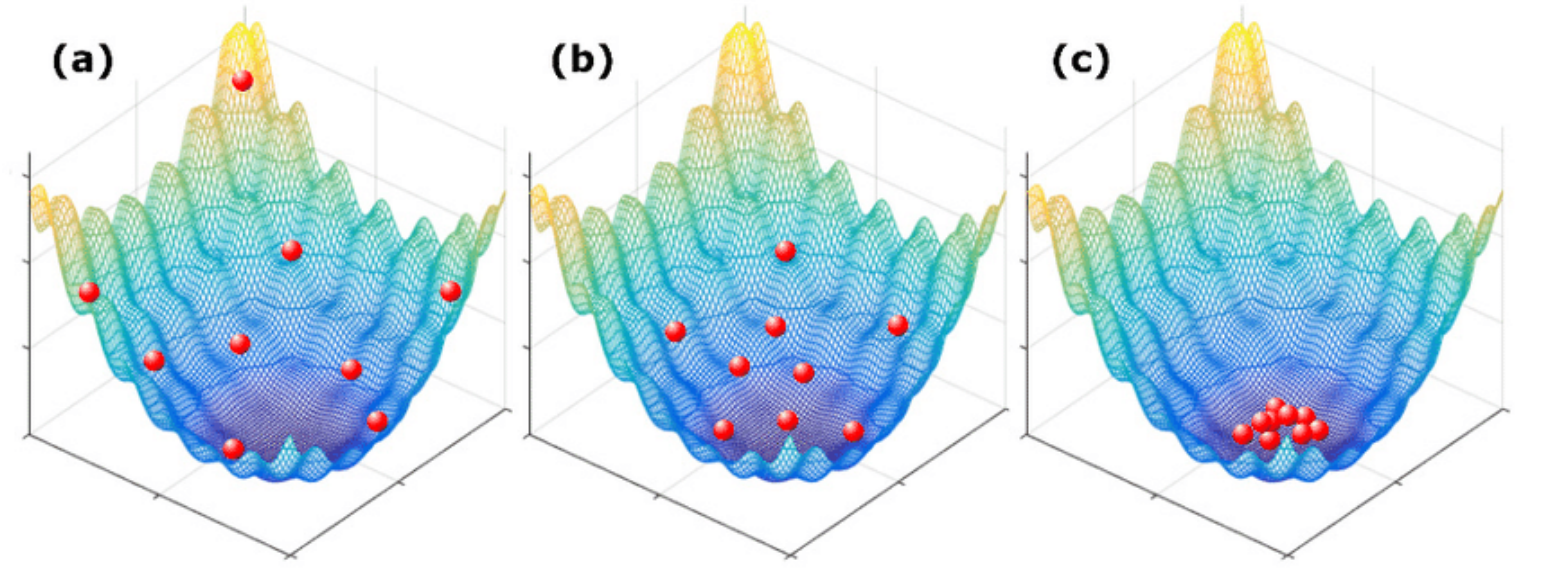
\includegraphics[width=3.5in]{images/Chap1/PSO.png}\\
        \caption{Particle Swarm Optimization \cite{R42}}
        \label{pso}
    \end{center}
\end{figure}

Defferential Evolution (DE) has been used in a hybrid algorithm along with PSO by Tand, B. et al. \cite{R43} to leverage 
both of the algorithms benefits. DE is rarely solely applied to path planning problems. In their review \cite{R37}
, of 20 years of research about DE, Bilal et al. did not mention robotics among the fields of application of DE. 
DE starts with a set of potential solutions. Each solution, or individual, is modified 
through mutation, crossover, and selection to improve over time. Mutation introduces random changes to create new 
candidates and avoid getting stuck in local optima. Crossover mixes parts of the new candidates with the original 
solutions to explore new possibilities. The selection process keeps only the better solutions for the next generation. 
This method effectively balances exploring new options and refining existing ones, making DE well-suited for complex 
optimization tasks.
By integrating improved PSO and DE algorithms for enhancing particle diversity, Tand, B. et al. achieved better 
path quality compared to other methods. The results demonstrate that their approach outperforms traditional 
evolutionary algorithms in path optimality an optimize computation times by 1.38\% \cite{R43}. 

Ant Colony Optimization (ACO) is known for being robust and good at parallel processing, but it can be slow and 
sometimes gets stuck in local optima solutions. To fix this, improvements like Ant Colony System (ACS) 
and Max-Min Ant System (MMAS) have been developed, which make ACO better at finding solutions but still have 
issues like being too rigid and converging too early. In mobile robot path planning, new strategies have been 
created to address these problems, such as adaptive methods that improve how pheromones are updated and balance 
exploration with finding the best path. Recent research has also introduced advanced versions like polymorphic 
ACO and multi-objective optimization, making ACO more effective for real-time and complex situations. However, 
these improvements also make the algorithm more complex and take more time to compute.

%advantages & limitations in discussion:

Meta-heuristic algorithms, such as Genetic Algorithms (GA), Particle Swarm Optimization (PSO), and Differential 
Evolution (DE), have become increasingly popular in robotic path planning. These algorithms are attractive because 
they can find good solutions to complex problems by mimicking natural processes like evolution or swarming behavior.
However, despite their growing use in research and their potential efficiency in practical usecases, the application 
of meta-heuristic algorithms in real-world robotic path planning like the intralogistics field remains quite limited. 
One of the major issues is that most studies focus on simulations rather than 
testing in real environments. While simulations can help develop and adjust these algorithms, they do not fully 
cover the challenges robots face in the real world, such as varying conditions, surface types, or unexpected 
noises. Another major issue is how obstacles are represented in these studies. Often, obstacles are either unrealistically 
large compared to the robot or have overly simple shapes that don’t accurately reflect real-world conditions. This 
lack of realism can result in algorithms that work well in simulations but fail when used in real environments. Additionally, 
because these algorithms are mostly tested in controlled, simulated settings, they may be too finely 
tuned to those specific conditions. This can make them less reliable when applied to the unpredictable conditions 
of the real world. In summary, while meta-heuristic algorithms show promise for robotic path planning, more real-world 
testing and realistic obstacle modeling are needed to ensure they work effectively in practical situations. 
Addressing these issues is key to advancing the use of robotics in intralogistics and other fields.
\newpage
\section{Summary and Discussion}
To synthesize the research conducted, it is paramount to summarize the key concepts comprehensively. This 
State of the Art report focuses on mobile robot path planning, a critical component of the overall 
robotic planning process. Effective path planning not only organizes and optimizes a robot's navigation 
but also significantly enhances its productivity by enabling it to execute missions more efficiently. 
In dynamic environments, a well-designed path planner is essential for ensuring safe operations and 
maximizing the robot's resource utilization and operational capacities. Moreover, Spline-based path planning represents a cutting-edge approach to achieving smooth and safe 
robot motion. This technique is particularly vital for managing heavy autonomous robots, such as 
forklifts, that handle sensitive materials and must operate with precision and stability. By utilizing 
constrained splines, it is possible to control various motion properties, including steering and 
the handling of abrupt turns, thereby reducing wear and tear on the robot and extending its operational 
lifespan. Nevertheless, there has to be a mean of quantifying the path qualities in order to test the 
performance of the used approach and to compare different approaches. This tool must be based on the 
properties of the path itself like length, direction changes, and clearance to obstacles.
These information are useful in a later stage to optimize the paths by optimizing the supervised 
properties of the paths. 

Meta-heuristic optimization algorithms are highly effective for refining mobile robot paths, particularly 
when building routes from scratch while considering both static and dynamic obstacles.
They also have the capability to solve problems without information about their mathematical model.
This has the great advantage of reducing the burden of expliciting the situation in order to solve it especially 
in complex cases where the effort to model the problem and the contsraints is higher and, later, the computation 
is harder. Instead, meta-heuristic algorithms focus on optimizing the fitness function related to the specific 
usecase. However, these algorithms are 
also computationally demanding due to their iterative nature, which involves repeatedly constructing and refining the path 
segments from the starting point to the end goal. Previously reviewed literature reveals that these algorithms often 
require significant computation 
time, which is acceptable in simulation environments but problematic in real-world applications. In a dynamic warehouse 
setting, blocking the area for extended periods to perform path planning is impractical. Such delays can disrupt 
warehouse operations, interfere with other vehicles and personnel, decrease overall productivity, and lead to 
increased time and energy costs. In addition the applications of meta-heuristic optimization approaches to robotics
in the intralogistics field is limited to mission scheduling and rarely tackles path planning problems.

Furthermore, the classical and the heuristic approaches are capable of creating new different paths every time the 
algorithms are ran even in the same environment setting. While this phenomenon proves of the intelligence of the algorithms
and the availability of several optimal paths, it makes the fully automated robot's behavior non-repeatable and unexplainable. 
For humans, it is difficult to foresee the behavior if many options are available. However, it is important for those working 
closely to robots to have an expectation of their behavior. It enables them to avoid collision risks and injuries and to 
plan their actions accordingly. If a predictable vehicle behavior is available, it promises a structured approach to path 
generation, reducing computational complexity and improving path quality.

Combining an optimal path planning approach that accomodates the kinematic constraints of Autonomous forklifts in the
intralogistics environment and generates smooth paths, is behaviorally explainable and deploys meta-heuristic Algorithms
is a new approach that would have an added value to mobile robot path planning in Intralogistics of reducing 
computation time and travel distance and improving AI driven solutions explainability. 




